\documentclass[a4paper,12pt, nofootinbib]{article}
\usepackage[width=15.5cm, left=3cm, top=3cm, right=2cm, left=2.5cm]{geometry}
\usepackage[spanish]{babel}
\usepackage[utf8]{inputenc}
\usepackage[T1]{fontenc}
\usepackage{xspace}
\usepackage{xargs}
\usepackage{fancyhdr}
\usepackage{lastpage}
\usepackage{caratula}
\usepackage[bottom]{footmisc}
\usepackage{amssymb}
\usepackage{algorithm}
\usepackage[noend]{algpseudocode}
\usepackage{placeins}
\usepackage[hidelinks]{hyperref}
\usepackage{xcolor}
\hypersetup{
      colorlinks,
      linkcolor={red!50!black},
      citecolor={blue!50!black},
      urlcolor={blue!80!black}
}


\usepackage{graphicx}
\usepackage{sidecap}
\usepackage{amsmath}
\usepackage{listings}


\lstset{ %
  frame=single,                    % adds a frame around the code
  keepspaces=true,                 % keeps spaces in text, useful for keeping indentation of code (possibly needs columns=flexible) 
  otherkeywords={*,...},            % if you want to add more keywords to the set
  numbers=left,                    % where to put the line-numbers; possible values are (none, left, right)
  numbersep=5pt,                   % how far the line-numbers are from the code
  showspaces=false,                % show spaces everywhere adding particular underscores; it overrides 'showstringspaces'
  showstringspaces=false,          % underline spaces within strings only
  showtabs=false,                  % show tabs within strings adding particular underscores
  stepnumber=1,                    % the step between two line-numbers. If it's4 1, each line will be numbered 
  tabsize=2,                     % sets default tabsize to 2 spaces
  title=\lstname                   % show the filename of files included with \lstinputlisting; also try caption instead of title
}

\setlength{\parindent}{4em}
\setlength{\parskip}{0.5em}


%%fancyhdr
\pagestyle{fancy}
\thispagestyle{fancy}
\addtolength{\headheight}{1pt}
\lhead{Sistemas Operativos: TP1}
\rhead{$2º$ cuatrimestre de 2015}
\cfoot{\thepage\ / \pageref{LastPage}}
\renewcommand{\footrulewidth}{0.4pt}

%\hypersetup{pdfpagemode=FullScreen}
\pdfcatalog{ /PageMode /FullScreen }

%%caratula
\materia{Sistemas Operativos}
\titulo{Trabajo Práctico Número 1}
\subtitulo{Scheduling}
%\grupo{Grupo 12}
%\integrante{Nombre}{LU}{email}
\integrante{Ciruelos Rodríguez, Gonzalo}{063/14}{gonzalo.ciruelos@gmail.com}
\integrante{}{}{}
\integrante{Thibeault, Gabriel}{114/13}{gabriel.eric.thibeault@gmail.com}

\begin{document}
\maketitle

\tableofcontents
\newpage

\section{Ejercicio 1}
\FloatBarrier
\par Nuestra implementaci\'on de la TaskConsola consiste en un ciclo que realiza $n$ (el primer par\'ametro de la tarea) interrupciones. 
Para determinar la cantidad de tiempo que debe durar cada interrupci\'on empleamos la funci\'on $std::rand()$ de la librer\'ia est\'andar. 
\par Sin embargo, es necesario normalizar el resultado de \'esta, ya que devuelve un valor entre $0$ y $RAND\_MAX$ (un macro definido en $stdlib.h$, dependiente de la implementaci\'on) y necesitamos que est\'e entre $bmin$ y $bmax$ (los otros dos par\'ametros de la tarea).
Para lograr esto, dividimos el valor aleatorio inicial por $RAND\_MAX - 0$, para obtener un n\'umero perteneciente al intervalo $[0, 1]$.
Luego, lo multiplicamos por $(bmax - bmin)+1$, obteniendo un resultado perteneciente al conjunto $[0, bmax - bmin + 1]$.
Finalmente sumamos $bmin$ y obtenemos un valor perteneciente al conjunto $[bmin, bmax + 1]$.
Si bien esto puede parecer incorrecto, el cast de un $double$ a un $int$ en C++ toma la parte entera del $double$, por lo que este conjunto es el deseado. 
\par El \'unico caso donde el resultado puede no llegar a ser el deseado es donde el valor es exactamente $bmax + 1$. 
Si bien esto no puede pasar en una variable continua (como ser\'ia te\'oricamente la uniforme que estamos manejando), al tratar con una representaci\'on de m\'aquina de los reales (como son los $doubles$) esto es posible (y sucede cuando $rand()$ devuelve exactamente $RAND\_MAX$).
Para evitar este error, si el resultado final es exactamente $bmax + 1$, le asignamos $bmax$.
\par En la figura \ref{fig:figuraEj1} se puede ver un ejemplo de un lote de tareas con dos Task Consolas (ambas con par\'ametros $n = 5$, $bmin = 1$ y $bmax = 3$).
\begin{figure}
\caption{Ejemplo de un lote de tareas con Task Consola}
\label{fig:figuraEj1}
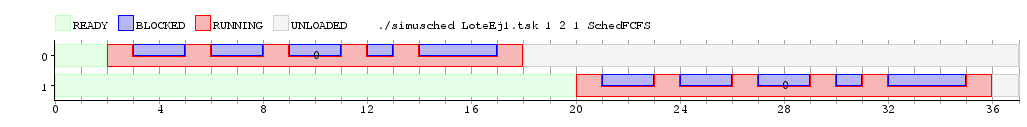
\includegraphics[width=0.9\columnwidth]{imgs/imgEj1.png}
\end{figure}
\FloatBarrier


\section{Ejercicio 2}

En las figuras \ref{fig:ej2-1core} y \ref{fig:ej2-2core} se pueden ver los gr\'aficos de Gantt para el lote de tareas de este ejercicio, para 1 y 2 cores, respectivamente.

La latencia para un solo core es de 4 ciclos de CPU para la taskCPU, 109 ciclos para una de las tasksConsola y 190 ciclos para la otra.
Para dos cores es de 4 ciclos para la taskCPU y una de las tasksConsola y de 85 para la otra.

Con los resultados de la figura \ref{fig:ej2-1core} se puede ver claramente el problema que puede surgir al utilizar un scheduler First Come First Serve: el usuario en este tipo de casos esperar\'ia poner a correr su algoritmo, y pasar el tiempo hasta que \'este termine de ejecutarse utilizando otras aplicaciones. 
Sin embargo, al correr este lote de tareas en una computadora con un solo core se debe esperar a que termine de correr la primer tarea para poder utilizar otras aplicaciones. 

Si bien con otro tipo de scheduler (por ejemplo Round Robin) el algoritmo tardar\'ia m\'as tiempo, el usuario podr\'ia utilizar otras aplicaciones mientras tanto para hacer pasar el tiempo.

Al emplear dos cores para correr el lote de tareas se alivia el problema detallado previamente, ya que al menos se puede ejecutar una de las aplicaciones deseadas mientras corre el algoritmo CPU-intensivo en el otro core, como se ve en la figura \ref{fig:ej2-2core}.
Sin embargo, el problema no se elimina completamente debido a que a\'un se debe esperar a que la primera aplicaci\'on termine de ejecutar para poder correr la segunda.

La \'unica forma de eliminar completamente este problema para un scheduler FCFS es tener a disposici\'on m\'as cores que tareas a ejecutar, pero s\'olo en raras circunstancias es posible satisfacer este requerimiento.

\begin{figure}[H]
\caption{Lote de tareas de Rolando para 1 core}
\label{fig:ej2-1core}
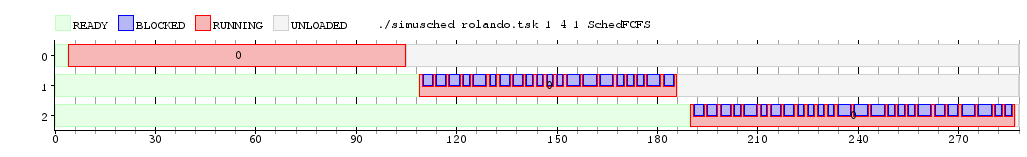
\includegraphics[width=1\textwidth]{imgs/ej2-1core}
\end{figure}

\begin{figure}[H]
\caption{Lote de tareas de Rolando para 2 cores}
\label{fig:ej2-2core}
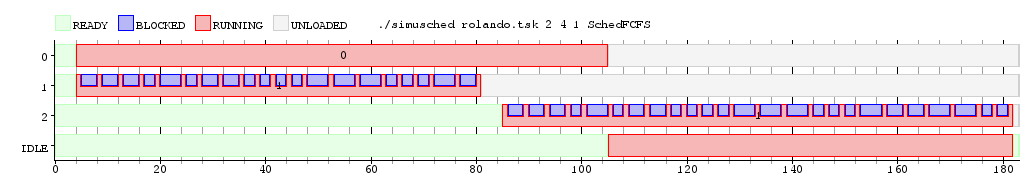
\includegraphics[width=1\textwidth]{imgs/ej2-2core}
\end{figure}



\section{Ejercicio 3}


Nuestra implementaci\'on de Task Batch consiste en crear un vector de bools de tama\~no $total\_cpu$ (el primer par\'ametro de la tarea), que se llena con $cant\_bloqueos$ valores en $true$ y el resto en $false$.
Luego, utilizamos el algoritmo de Fisher-Yates para hacer un shuffle del vector.
Finalmente, se lo recorre, y por cada posici\'on, si el valor es $true$ se hace una interrupci\'on de IO, y si es $false$ se hace uso de la CPU.

En la figura \ref{fig:figuraEj3} se puede ver un lote de tareas con 3 TaskBatch, con par\'ametros 5 y 2; 28 y 19; 14 y 13.

\begin{figure}[H]
\caption{Ejemplo de un lote de tareas con Task Batch}
\label{fig:figuraEj3}
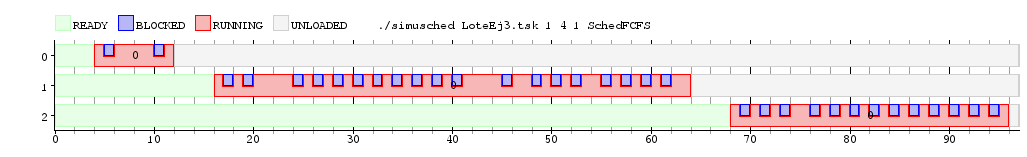
\includegraphics[width=1\textwidth]{imgs/imgEj3.png}
\end{figure}



\section{Ejercicio 4}
\par Para implementar el scheduler Round-Robin, decidimos usar en la estructura privada de la clase SchedRR una cola global con los pids de los procesos(ints), y dos vectores del tamaño de la cantidad de cores, uno para guardar el valor de los quantums correspondiente a cada core, y el otro para almacenar el tiempo restante hasta el desalojo, que se irá decrementando con los ticks.

\par Los algoritmos son simples:

\begin{itemize}
\item Para inicializar el scheduler, inicializamos con una cola vacía, y el vector de quantums y time\_left con los valores correspondientes a los valores de quantum de cada core, pasados por parámetro.
\item \emph{load} simplemente pushea un pid a la cola de procesos.
\item \emph{unblock}, al igual que load, agrega el proceso desbloqueado a la cola global.
\item En cada \emph{tick}, se evalúa el Motivo pasado por parámetro. En caso de que el proceso haya terminado (m==EXIT), si no hay procesos por ejecutar, se regresa a la tarea Idle, de lo contrario, se reinicia el timeleft del core al valor inicial (el valor de los quantum de dicho core) y pasa a ejecutar el primer proceso en la cola. En caso de que el proceso se encuentre bloqueado (m==BLOCK), al igual que en el caso anterior, se pasa a ejecutar el próximo proceso (el pid del proceso bloqueado recién regresará a la cola cuando se desbloquee). Por último, si no se cumplen estas condiciones (no terminó ni está bloqueado), si se está ejecutando la tarea idle, chequea que no haya procesos en la cola, y en caso de que lo haya le otorga la ejecución al primero. Si no fuera la tarea idle la que se está ejecutando, se resta uno al timeleft, y si éste llega a 0, se pasa a ejecutar el próximo proceso en la cola, reiniciando el valor del timeleft al valor de quantum original.
\end{itemize}

\section{Ejercicio 5}

\begin{figure}[H]
\caption{Lote de tareas ejecutando con Round Robin con quantum 2}
\label{fig:ej5q2}
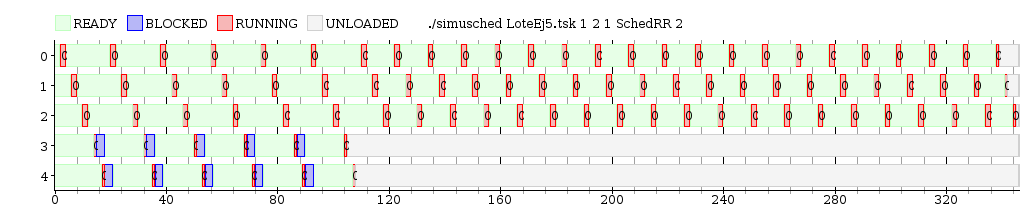
\includegraphics[width=1\textwidth]{imgs/ej5-q2.png}
\end{figure}

\begin{figure}[H]
\caption{Lote de tareas ejecutando con Round Robin con quantum 10}
\label{fig:ej5q10}
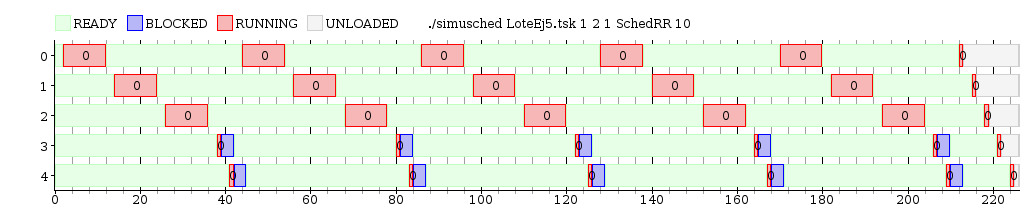
\includegraphics[width=1\textwidth]{imgs/ej5-q10.png}
\end{figure}

\begin{figure}[H]
\caption{Lote de tareas ejecutando con Round Robin con quantum 50}
\label{fig:ej5q50}
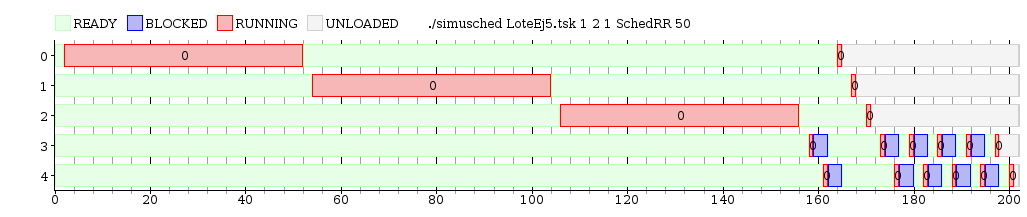
\includegraphics[width=1\textwidth]{imgs/ej5-q50.png}
\end{figure}

\begin{center}
  \begin{tabular}{ c c}
Tarea 0
\begin{tabular}{| l | c | c | c |}
\hline  
\textbf{Quantum} & \textbf{2} & \textbf{10} & \textbf{50} \\ \hline
Latencia & 2 & 2 & 2 \\ \hline
Waiting Time & 288 & 162 & 114 \\ \hline
Tiempo Total & 339 & 213 & 165 \\ \hline
\end{tabular}&


Tarea 1
\begin{tabular}{| l | c | c | c |}
\hline  
\textbf{Quantum} & \textbf{2} & \textbf{10} & \textbf{50} \\ \hline
Latencia & 6 & 14 & 54 \\ \hline
Waiting Time & 291 & 165 & 117 \\ \hline
Tiempo Total & 342 & 216 & 168 \\ \hline
\end{tabular} \\[3em]

Tarea 2
\begin{tabular}{| l | c | c | c |}
\hline  
\textbf{Quantum} & \textbf{2} & \textbf{10} & \textbf{50} \\ \hline
Latencia & 10 & 26 & 106 \\ \hline
Waiting Time & 294 & 168 & 120 \\ \hline
Tiempo Total & 345 & 219 & 171 \\ \hline
\end{tabular} &



Tarea 3 
\begin{tabular}{| l | c | c | c |}
\hline  
\textbf{Quantum} & \textbf{2} & \textbf{10} & \textbf{50} \\ \hline
Latencia & 14 & 38 & 158 \\ \hline
Waiting Time & 84 & 201 & 177 \\ \hline
Tiempo Total & 105 & 222 & 198 \\ \hline
\end{tabular} \\[3em]

Tarea 4
\begin{tabular}{| l | c | c | c |}
\hline  
\textbf{Quantum} & \textbf{2} & \textbf{10} & \textbf{50} \\ \hline
Latencia & 17 & 41 & 161 \\ \hline
Waiting Time & 87 & 204 & 180 \\ \hline
Tiempo Total & 108 & 225 & 201 \\ \hline
\end{tabular} & \\

\end{tabular}

\end{center}

\hspace{4em}

\begin{figure}[H]
\caption{Valores Promedio entre las tareas}
\label{fig:ej5-tabla}
\begin{center}
\begin{tabular}{| l | c | c | c |}
\hline  
\textbf{Quantum} & \textbf{2} & \textbf{10} & \textbf{50} \\ \hline
Latencia & 9.8 & 24.2 & 96.2 \\ \hline
Waiting Time & 208.8 & 180 & 141.6 \\ \hline
Tiempo Total & 247.8 & 219 & 180.6 \\ \hline
\end{tabular}
\end{center}
\end{figure}

Conclusiones a partir de los gráficos (figuras \ref{fig:ej5q2}, \ref{fig:ej5q10} y \ref{fig:ej5q50}, además de la tabla de la figura \ref{fig:ej5-tabla}): 

\begin{itemize}

\item Con respecto a la \textbf{latencia}, es menor en el caso con el scheduler con quantum de 2 ciclos. Esto se debe a que el primer desalojo se hace más rápido ya que el tiempo asignado por quantum es menor que en los demás. Como se ve en la tabla de los promedios, el valor de la latencia aumenta cuanto mayor es el valor del quantum.
\item Con respecto al \textbf{waiting time}, ocurre lo contrario, es menor con el scheduler de quantum 50. Esto se debe a que cuanto menor es el quantum, más cambios de contexto se realiza durante la ejecución de las tareas, y esto agrega tiempo de espera ya que cada cambio de contexto tarda 2 ciclos en realizarse.
\item Por último, el \textbf{tiempo total}, al igual que en el anterior, es menor en último caso, con quantum de 50 ciclos. De la misma manera, al aumentar el quantum y reducir los cambios de contexto, y por ende los costos de cada cambio de contexto, el tiempo total se reduce.
\end{itemize}





\section{Ejercicio 6}

\begin{figure}[H]
\caption{Lote de tareas ejecutando con FCFS}
\label{fig:ej6}
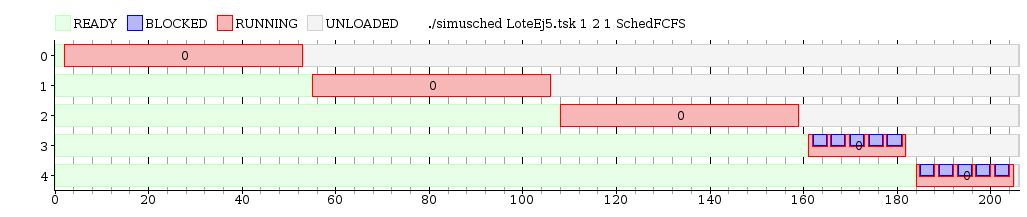
\includegraphics[width=1\textwidth]{imgs/ej6.png}
\end{figure}


\section{Ejercicio 7}

Primero, lo que hicimos fue testear cuando se le pasaban muchos parámetros.

\begin{figure}[H]
\caption{Ejemplo de un lote de tareas con Task Consola}
\label{fig:ej71}
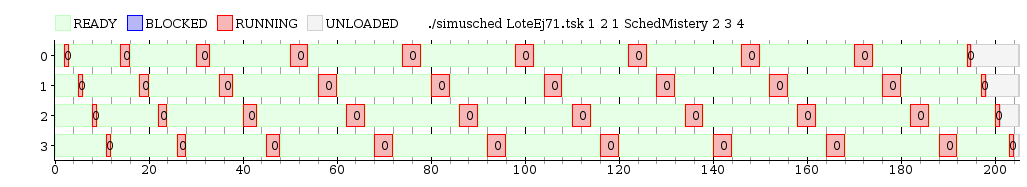
\includegraphics[width=1\textwidth]{imgs/ej7-1.png}
\end{figure}

Como se vé en la imagen, la cantidad de parámetros determina cuanto va a ser el quantum que se le asigna a cada tarea, progresivamente. Además gracias a este test, pudimos ver que hay preemption, y que el método probablemente sea similar a Round Robin.


Luego, lo que hicimos fue ver que pasa si una tarea se bloquea.

\begin{figure}[H]
\caption{Ejemplo de un lote de tareas con Task Consola}
\label{fig:ej72}
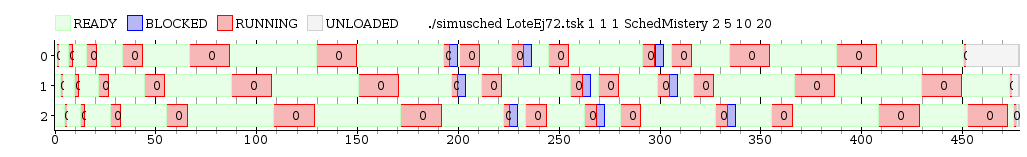
\includegraphics[width=1\textwidth]{imgs/ej7-2.png}
\end{figure}

Gracias a esta imagen pudimos confirmar que hay una idea de prioridades detrás de este scheduler. Esto se debe a que cuando una tarea se desbloquea, tiene \emph{más prioridad}, dado que por ejemplo, la tarea 0, despues de desbloquearse, se ejecuta antes que la tarea 2, que era la que a priori le tocaba, si se tratara de un Round Robin común y corriente.

Además, este test nos permitió ver que cuando una tarea se desbloquea va a la cola que le sigue en prioridad (de más prioridad).


Entonces, de esta manera confirmamos que se trata de un scheduling de prioridad, en el que hay $n$ colas (si nos pasaron $n-1$ parámetros), donde cada cola tiene un quantum igual al parámetro que corresponde (o 1 si es la primera). Y lo que hace el algoritmo es ir por la lista de colas buscando alguna cola no vacía, y si encuentra alguna no vacía corre la próxima tarea que corresponda.

Además, cuando una tarea es desalojada, pasa a estar en la cola siguiente (de menor prioridad) que la que estaba antes, y si estaba en la de menos prioridad se queda en esa.

En cuanto a la implementación, tenemos un vector de colas, y un vector de quantums (cuanto es el quantum de cada cola de tareas). Además, tenemos un entero que nos indica cuanto tiempo le queda a la tarea actual y de que cola salió.

Entonces, cuando cargamos una tarea la ponemos en la cola mas prioritaria. Cuando una tarea se desbloquea, la ponemos en la cola anterior (de más prioridad). Cuando una tarea debe ser desalojada porque se acabó el tiempo que se le asignó, se recorre el vector de colas buscando la primera no vacía y en caso de que la encuentre, popea un pid y lo pone a correr. En caso de que no encuentre, continúa corriendo la tarea actual.



\section{Ejercicio 8}


Para implementar este scheduler, debemos mantener $n$ cantidad de colas, donde $n$ es la cantidad de cores del procesador. Además, como cuando entra un proceso nuevo debemos asignarlo al procesador con menos procesos totales, nos conviene tener un vector que nos dice cuantos procesos totales tiene cada core. Como siempre, tenemos los quantums de cada procesador, y el tiempo restante que tiene cada tarea de cada core. 

Finalmente, tenemos un diccionario, cuyas claves son tareas y sus significados son cores, que nos dice para cada proceso bloqueado, a que core le corresponde. Necesitamos esto para sabes, cuando un proceso se desbloquea, a que core asignarselo.

Entonces, cuando entra un nuevo proceso, buscamos cual es el core con menos procesos actuales, y lo asignamos ahí. Cuando un proceso termina, lo que hacemos es fijarnos en la cola de cada core cual es el proceso que sigue.

Cuando un proceso se bloquea, lo definimos en el diccionario nombrado anteriormente; y cuando se desbloquea, buscamos en el diccionario a que core tiene que ir y borramos su entrada.

\subsection{Escenario 1}

La versión de Round Robin que no migra nucleos es beneficiosa en conjuntos de tareas que usan intensivamente el CPU y la memoria durante mucho tiempo. Como la memoria se usa intensivamente, migrar cores es costoso porque se pierde todo lo que estaba cacheado. 

El lote que diseñamos consiste en 3 tareas, cada una empieza un segundo despues de la otra, y cada una usa el procesador por 30 unidades de tiempo.

\begin{lstlisting}
TaskCPU 30
@1:
TaskCPU 30
@2:
TaskCPU 30
\end{lstlisting}


\begin{figure}[H]
\caption{Ejemplo de un lote de tareas que solo usa CPU en Round Robin 1}
\label{fig:ej8-11}
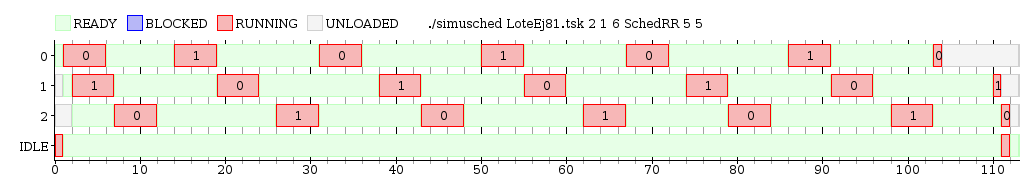
\includegraphics[width=1\textwidth]{imgs/ej8-1rr.png}
\end{figure}

\begin{figure}[H]
\caption{Ejemplo de un lote de tareas que solo usa CPU en Round Robin 2}
\label{fig:ej8-12}
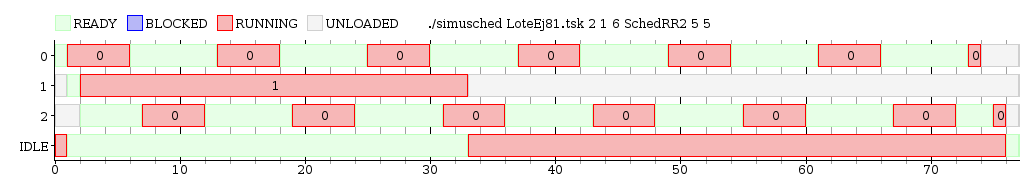
\includegraphics[width=1\textwidth]{imgs/ej8-1rr2.png}
\end{figure}

Las métricas que analizaremos serán la eficiencia (tiempo en el que el cpu está corriendo las tareas sobre tiempo total) y el throughput.

Como se ve en la figura \ref{fig:ej8-11}, la eficiencia de el algoritmo de scheduling que migra nucleos no es tan alta, dado que la migración de nucleos ocurre muy seguido y se debe pagar un costo muy alto cada vez. Por esta misma razón, el throughput de este algoritmo es también bajo.

Por otro lado, como se ve en la figura \ref{fig:ej8-12}, la eficiencia de el algoritmo de scheduling que no migra nucleos (si no fuera por el idle del final, que se solucionaria simplemente poniendo igual cantidad de tareas en cada nucleo) es mucho más alta. Esto se debe a que al no migrar nucleos, se aprovecha el cache del core y no es se paga el costo de perderlo. Por esta razón, el throughput del algoritmo es más alto que antes, terminando las tareas en casi la mitad del tiempo que el anterior algoritmo.

\subsection{Escenario 2}

Ahora veamos que pasa si hay una tarea que se bloquea por mucho tiempo, una que lo usa por muy poco tiempo y otras 2 que requieren usar CPU por un poco más de tiempo.

\begin{lstlisting}
TaskIO 1 70
TaskCPU 50
@1:
TaskCPU 5
TaskCPU 50
\end{lstlisting}

\begin{figure}[H]
\caption{Ejemplo de un lote de tareas que se bloquean y usan CPU en Round Robin 1}
\label{fig:ej8-21}
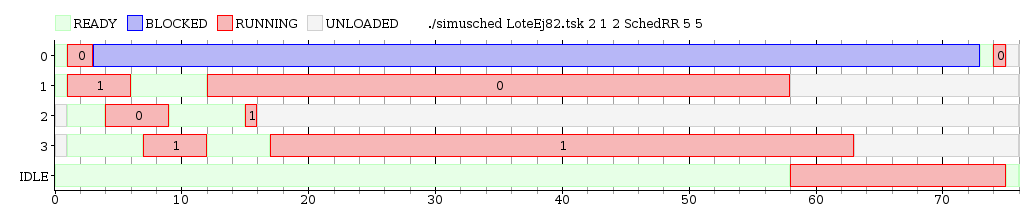
\includegraphics[width=1\textwidth]{imgs/ej8-2rr.png}
\end{figure}

\begin{figure}[H]
\caption{Ejemplo de un lote de tareas que se bloquean y usan CPU en Round Robin 2}
\label{fig:ej8-22}
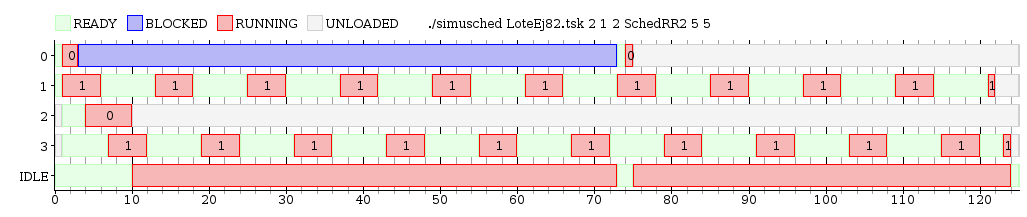
\includegraphics[width=1\textwidth]{imgs/ej8-2rr2.png}
\end{figure}


Como se ve en la figura \ref{fig:ej8-21}, el rendimiento y el throughput de esta versión es altisimo. Esto se debe a que, cuando se bloquea un proceso, el algoritmo puede correr en paralelo las 2 tareas demandantes de CPU en paralelo totalmente.

Sin embargo, en la versión del algoritmo que no permite migración entre procesadores, en la figura \ref{fig:ej8-22} todo cambia. Al no poder migrar tareas entre núcleos, cuando la tarea 2 termina, y la tarea 0 está bloqueada, el procesador 1 tiene una carga muy alta, mientras que el procesador 0 esta totalmente ocioso. Por esta razón, la eficiencia es mucho más baja que antes, y en consecuencia, el throughput es mucho más bajo.





\end{document}
